\chapter{Motivation}
\label{ch:motivation}

Static analysis plays a prominent role in releasing bug-free software. In spite of that, important tools suffer from well-documented usability issues \cite{CB16,JSMB13}. Johnson et. al. \cite{JSMB13}  found design flaws in current static analysis tools and the need for an interactive mechanism in assisting developers in fixing bugs. They conducted interview with 20 participants of which 16 are professional developers and 4 are graduate students. The interesting findings are like if the output of static analysis tool is user friendly and intuitive then false positives and high number of warnings could be less problematic for a developer, showing call hierarchies with which parts of code are affected by a bug, be able to share settings with predefined coding standards among the team, need of a web browser for reacting on the analysis output for instance adding comment to a bug which goes out of context to the developer. Christakis et. al. \cite{CB16} also did an empirical study on what developers want and need from program analysis. They did a survey by sending invitations to 2,000 developers within their organisation i.e., Microsoft and received 375 responses. The resultant data is analysed and found that there are some obstacles which hinder the usage of a static analysis tool by a developer such as 'Wrong checks are on by default', 'Too many false positives', 'Too slow',  'Complex user interface' etc. Being a user interface an obstacle for a developer along with other usability problems is noteworthy. The key takes away from the above-mentioned papers is the importance of Usability in the ongoing adaption of static analysis tools. \\ \\ 

In general, the setup of most of the recent research \cite{CB16} \cite{JSMB13} done in the area of Static Code Analysis is like assuming a single project in an organisation. Further, they assume there is a single person working on a single project with a single tool tackling a single type of problems.  Somehow, the assumptions are made so singular to address a specific issue in their research. However, in practice i.e., in the real world of software engineering, there are numerous people working in teams for multiple projects at a time. Each project uses multiple tools in their software development. Even in the case of Static Code Analysis, multiple tools are used which are each capable of addressing several types of issues in order to find more code flaws \cite{SCALe}. \\ \\


\section{Current Research in Using Multiple Analysis Tools}

In the current research, we could see the usage of multiple tools in the software industry where each tool is different in computation approaches as one could be standard run on Nightly builds for example with Checkmarx \cite{checkmarx} tool or could be following Incremental Analysis, which means only testing the changed version of code instead of running analysis on complete codebase. The reasons of using multiple tools could be as each tool is capable of detecting bugs with different coverage \cite{bessey2010few} \cite{delaitre2015evaluating}, it could help in finding more bugs easily which are not found by tool but the other \cite{plakosh2014improving}. There is also research \cite{flynn2018prioritizing} going in the direction of using multiple static analysis tools in order to prioritise the bug warning alerts. There is a paper \cite{meng2008approach} published in 2008 which uses results of three different static analysis tools for a programming language, Java and merges them together in order to show warnings to the developer. \\ \\

Caitlin et. al. and team developed a framework called Tricorder \cite{tricorder} which mentions about using multiple tools where each tool covers separate bug coverage. The results are displayed during the code review and published by a bot called ReviewBot. The evaluation is made as a summative approach using click rates by the user which shows which tool is better in comparison to others. Cristina et. al. and team developed a framework called Parfait \cite{parfait} using multiple tools which address the issues with scalability and precision. For scalability, it checks the easy and expensive analysis for each bug type and for precision it tracks each bug whether it is real, potential or not. \\ \\

Although we have seen the current research trends and their direction, the usability aspect is not addressed so far in the context of using multiple tools. There are no research papers found addressing the usability issue with multiple tools in single interface. The multiplicity of tools used for a single project and that too with different computation capabilities brings a new challenge.  One tool could produce results in no time and others could take more time in comparison. This could lead to a situation of breaking the usability of the user interface. On that challenge, this thesis aims to address such a scenario with a problem statement as " How to integrate the results of multiple static analysis tools in a unified user interface? ".  \\ \\

The thesis work begins by brainstorming on the problem statement and as a result, different research questions are brought up and of which three research questions are selected with respect to available sources, scope and limitations of thesis time frame. \\ \\

\section{What Current Tools do?}

Let us now examine each research question and see what the current tools behave like. \\ \\

\textbf{1. How to display the results of the same codebase from different analysis tools?}  \\

This question needs to address the scalability aspect of displaying results as usage of multiple tools results in redundancy and a high number of warnings with more coverage. The following \autoref{fig:findbugs-results} shows how a FindBugs \cite{findbugs} static analysis tool shows results for a project \cite{findbugs-example}. This could be the same with other tool and so when you use multiple tools, there is a need for a better user interface.\\ \\

\begin{figure}[hbt!]
	\centering
	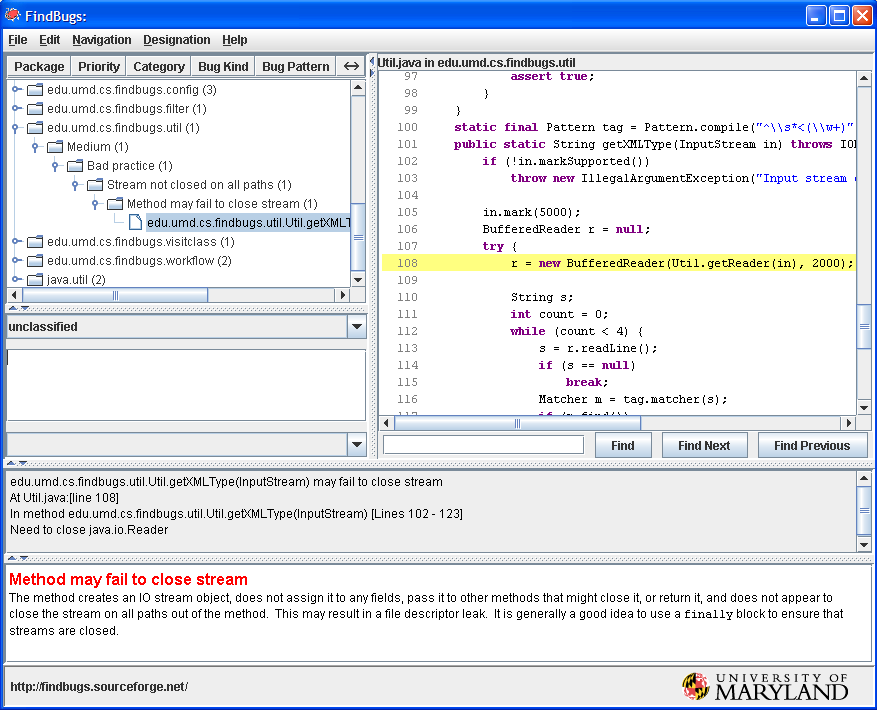
\includegraphics[width=\linewidth]{figures/findbugs-results}
	\caption{A preview of FindBugs scan results.}
	\label{fig:findbugs-results}
\end{figure}

\clearpage

The Tricorder shows the results with multiple tools as seen in the following \autoref{fig:tricorder-results} where two findings each from different tool. \\ \\

\begin{figure}[hbt!]
	\centering
	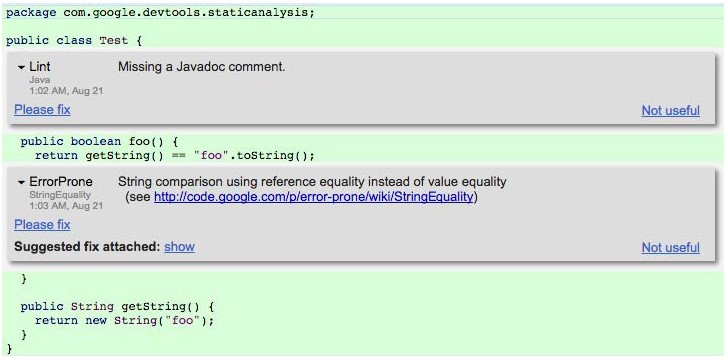
\includegraphics[width=\linewidth]{figures/Tricorder}
	\caption{A preview of Tricorder scan results. \cite{tricorder}}
	\label{fig:tricorder-results}
\end{figure}

\textbf{2. What feedback works to know that the bug fixing is on-going?} \\

This question needs to address the scenario where one tool could give an instant update on the bug fixing process and others might take more time to analyse and report the update on it. In the design aspect, especially the User Interface needs to be adaptive \cite{NB18} enough as static analysis tools sometimes take a long time to stop and there is no intuitive feedback provided. Also, One interesting aspect of Johnson et. al. \cite{JSMB13} study is about the importance of feedback from tools without disrupting the developer workflow. Traditionally, the project files are added to FindBugs \cite{findbugs} tool as seen in the \autoref{fig:findbugs-scan} in order to start the scanning and the user has to wait for some minutes to see the results. There was no feedback in the process of scanning. \\ \\

\begin{figure}[hbt!]
	\centering
	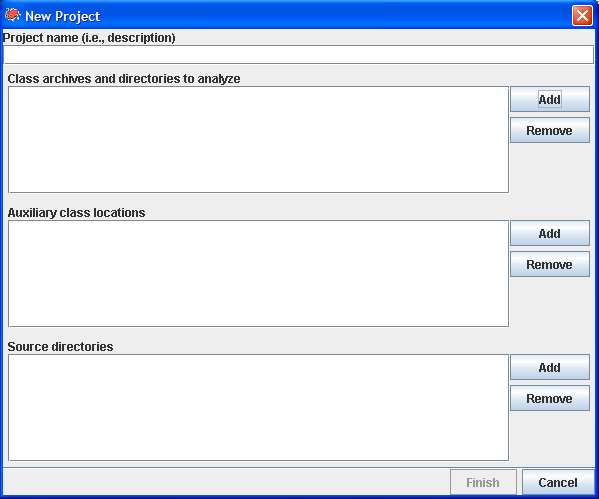
\includegraphics[width=\linewidth]{figures/findbugs-scan}
	\caption{A preview of initiating FindBugs to scan a project. \cite{findbugs}}
	\label{fig:findbugs-scan}
\end{figure}

Back in the history of Computer Science, there is an observation made when the user interface is non-responsive, the user shuts down the system. Thereafter, comes to the implementation of user interface called Ghost screen by Colleran et al. \cite{colleran} who patented the method which manages application programs with non-responsive user interfaces in the year 2005. About the response times, NN Group \cite{nn} states that if the execution of a certain task takes 0.1 up to 1 second then there is no need for feedback, just show the result. If it takes 10 seconds, there should be feedback and if it is variable every time then there is the importance of per cent bar \cite{Borman} but sometimes it could be overkill to use as it cause stress to the user by the principle of display inertia. If the time taken by a task is unknown then there has to be feedback like a spinning ball or in an example of a task being to scan databases then it has to report user what database is being scanned currently. Overall, there has to be feedback stating that the system is working, if not indicating what is actually doing. This motivates to know how responsiveness in terms of usability is vital to consider in the development of modern tools. Further, this needs to be addressed in the context of using multiple tools.\\ \\


\textbf{3. How to carry traceability of bug fixing?} \\

In the scenario, where the user has picked a bug to fix and worked on it and later he submitted for analysis. Then the bug could either get fixed or new bugs could have been introduced or different bugs got resolved by fixing the one bug. All these might have taken place and this is uncertain. Thereby it would be better to have traceability in order to somehow safeguard the code repository from future bugs or monitor the changes happening in the context of bugs. \\ \\

As per the related work in research \cite{heinemann2014teamscale}, a tool named "Teamscale" \cite{teamscale} shows the influence on the quality status for each change in code backed by version control commits. For a change, it shows how many quality problems are added or removed. The illustration could be observed in the following \autoref{fig:teamscale}.\\ \\

\begin{figure}[hbt!]
	\centering
	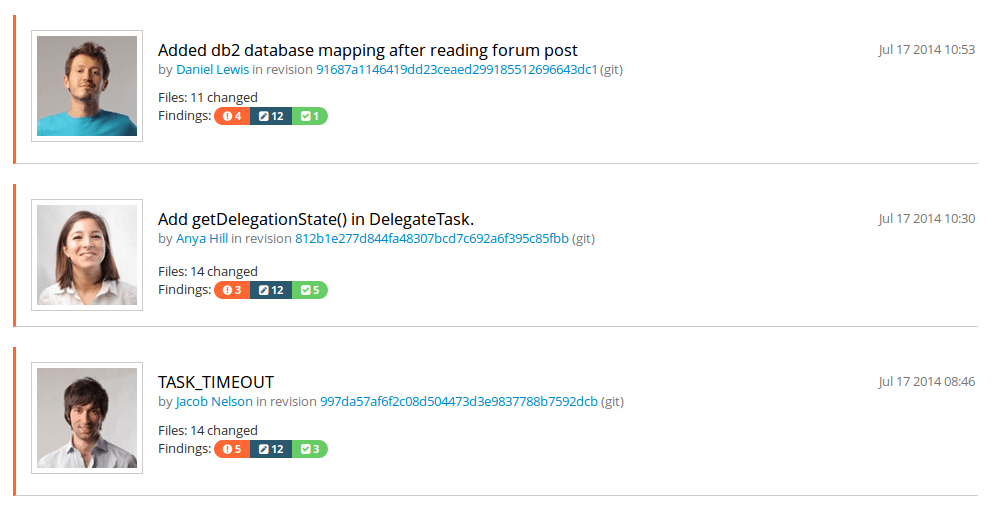
\includegraphics[width=\linewidth]{figures/teamscale}
	\caption{A Teamscale feature of showing quality status with code changes. \cite{teamscale}}
	\label{fig:teamscale}
\end{figure}

\let\cleardoublepage\clearpage
